%%%%%%%%%%%%%%%%%%%%%%%%%%%%%%%%%%%%%%%%%
% Beamer Presentation
% LaTeX Template
% Version 1.0 (10/11/12)
%
% This template has been downloaded from:
% http://www.LaTeXTemplates.com
%
% License:
% CC BY-NC-SA 3.0 (http://creativecommons.org/licenses/by-nc-sa/3.0/)
%
%%%%%%%%%%%%%%%%%%%%%%%%%%%%%%%%%%%%%%%%%

%----------------------------------------------------------------------------------------
%	PACKAGES AND THEMES
%----------------------------------------------------------------------------------------

\documentclass{beamer}
\usepackage{paquete}
\mode<presentation> {

% The Beamer class comes with a number of default slide themes
% which change the colors and layouts of slides. Below this is a list
% of all the themes, uncomment each in turn to see what they look like.

%\usetheme{default}
%\usetheme{AnnArbor}
%\usetheme{Antibes}
%\usetheme{Bergen}
%\usetheme{Berkeley}
%\usetheme{Berlin}
%\usetheme{Boadilla}
%\usetheme{CambridgeUS}
%\usetheme{Copenhagen}
%\usetheme{Darmstadt}
%\usetheme{Dresden}
%\usetheme{Frankfurt}
%\usetheme{Goettingen}
%\usetheme{Hannover}
%\usetheme{Ilmenau}
%\usetheme{JuanLesPins}
%\usetheme{Luebeck}
\usetheme{Madrid}
%\usetheme{Malmoe}
%\usetheme{Marburg}
%\usetheme{Montpellier}
%\usetheme{PaloAlto}
%\usetheme{Pittsburgh}
%\usetheme{Rochester}
%\usetheme{Singapore}
%\usetheme{Szeged}
%\usetheme{Warsaw}

% As well as themes, the Beamer class has a number of color themes
% for any slide theme. Uncomment each of these in turn to see how it
% changes the colors of your current slide theme.

%\usecolortheme{albatross}
%\usecolortheme{beaver}
%\usecolortheme{beetle}
%\usecolortheme{crane}
%\usecolortheme{dolphin}
%\usecolortheme{dove}
%\usecolortheme{fly}
%\usecolortheme{lily}
%\usecolortheme{orchid}
%\usecolortheme{rose}
%\usecolortheme{seagull}
%\usecolortheme{seahorse}
%\usecolortheme{whale}
%\usecolortheme{wolverine}

%\setbeamertemplate{footline} % To remove the footer line in all slides uncomment this line
%\setbeamertemplate{footline}[page number] % To replace the footer line in all slides with a simple slide count uncomment this line

%\setbeamertemplate{navigation symbols}{} % To remove the navigation symbols from the bottom of all slides uncomment this line
}

\usepackage{graphicx} % Allows including images
\usepackage{booktabs} % Allows the use of \toprule, \midrule and \bottomrule in tables

%----------------------------------------------------------------------------------------
%	TITLE PAGE
%----------------------------------------------------------------------------------------

\title[Bomberman]{TPI Bomberman} % The short title appears at the bottom of every slide, the full title is only on the title page

\author{Grupo Ford Fiesta} % Your name
\institute[UTN FRBA] % Your institution as it will appear on the bottom of every slide, may be shorthand to save space
{
Universidad Tecnológica Nacional -FRBA \\ % Your institution for the title page
\medskip
\textit{Tobias Duren} % Your email address
\newline
\textit{Jose Miguel Paz Portilla} % Your email address
\newline
\textit{Lucas Ezequiel Fernandez Fiel} % Your email address
}
\date{\today} % Date, can be changed to a custom date

\begin{document}

\begin{frame}
\titlepage % Print the title page as the first slide
\end{frame}

\begin{frame}
\frametitle{INDICE} % Table of contents slide, comment this block out to remove it
\tableofcontents % Throughout your presentation, if you choose to use \section{} and \subsection{} commands, these will automatically be printed on this slide as an overview of your presentation
\end{frame}

%----------------------------------------------------------------------------------------
%	PRESENTATION SLIDES
%----------------------------------------------------------------------------------------

%------------------------------------------------
\section{Personajes} % Sections can be created in order to organize your presentation into discrete blocks, all sections and subsections are automatically printed in the table of contents as an overview of the talk
%------------------------------------------------

\subsection{Bomberman Blanco} % A subsection can be created just before a set of slides with a common theme to further break down your presentation into chunks
\subsection{Bomberman Negro}

\begin{frame}
\frametitle{Bomberman}
El juego tiene hasta 2 personajes que colocan bombas, cada uno inicia con 3 vidas y su bomba se expande hasta un cuadro desde donde se ubico la bomba.
\begin{figure}[H]
	\centering
	
\includegraphics[scale=0.3]{assets/bomberman1/bomberman1frente.png}
    \caption{Bomberman blanco.}
    \label{fig:bombermanBranco}
\end{figure}  
\begin{figure}[H]
	\centering
	
\includegraphics[scale=0.3]{assets/bomberman2/bomberman2frente.png}
    \caption{Bomberman negro.}
    \label{fig:bombermanNegro}
\end{figure} 

\end{frame}

%------------------------------------------------

%\begin{frame}
%\frametitle{Bullet Points}
%\begin{itemize}
%\item Lorem ipsum dolor sit amet, consectetur adipiscing elit
%\item Aliquam blandit faucibus nisi, sit amet dapibus enim tempus eu
%\item Nulla commodo, erat quis gravida posuere, elit lacus lobortis est, quis porttitor odio mauris at libero
%\item Nam cursus est eget velit posuere pellentesque
%\item Vestibulum faucibus velit a augue condimentum quis convallis nulla gravida
%\end{itemize}
%\end{frame}

%------------------------------------------------

%\begin{frame}
%\frametitle{Blocks of Highlighted Text}
%\begin{block}{Block 1}
%Lorem ipsum dolor sit amet, consectetur adipiscing elit. Integer lectus nisl, ultricies in feugiat rutrum, porttitor sit amet augue. Aliquam ut tortor mauris. Sed volutpat ante purus, quis accumsan dolor.
%\end{block}

%\begin{block}{Block 2}
%Pellentesque sed tellus purus. Class aptent taciti sociosqu ad litora torquent per conubia nostra, per inceptos himenaeos. Vestibulum quis magna at risus dictum tempor eu vitae velit.
%\end{block}

%\begin{block}{Block 3}
%Suspendisse tincidunt sagittis gravida. Curabitur condimentum, enim sed venenatis rutrum, ipsum neque consectetur orci, sed blandit justo nisi ac lacus.
%\end{block}
%\end{frame}

%------------------------------------------------


%------------------------------------------------
\section{Enemigos}
\subsection{Enemigo común}
\subsection{Enemigo jefe}
\begin{frame}
\frametitle{Enemigos}

Tambien cuenta con enemigos que si tocan a los personajes lo matan. Hay enemigos comunes y enemigo jefe que cuenta con 5 vidas y atraviesa paredes.

\begin{figure}[H]
	\centering
	
\includegraphics[scale=0.3]{assets/rivales/rivalfrente.png}
    \caption{Rival común.}
    \label{fig:rivalComun}
\end{figure}  
\begin{figure}[H]
	\centering
	
\includegraphics[scale=0.3]{assets/rivales/bossfrente.png}
    \caption{Rival Jefe.}
    \label{fig:rivalJefe}
\end{figure} 

\end{frame}

\section{Power Up}
\subsection{Vida extra}
\subsection{Bomba extra}
\subsection{Bomba atraviesa paredes}
\subsection{Incremento de alcance de la bomba}
\begin{frame}
\frametitle{Power Up}
Hay cuatro power up en el juego que permiten aumentar habilidades de los jugadores y se encuentran ocultos bajo los ladrillos. Estos permiten aumentar una vida, una bomba, una unidad de alcance de la bomba o bien permite atravesar una pared para matar a un enemigo.

\begin{figure}[H]
	\centering
	
\includegraphics[scale=0.2]{assets/powerups/vidaextra.png}
    \caption{Vida extra.}
    \label{fig:vida extra}
\end{figure} 

\begin{figure}[H]
	\centering
	
\includegraphics[scale=0.2]{assets/powerups/bombaextra.png}
    \caption{Bomba extra.}
    \label{fig:bomba extra}
\end{figure} 

\begin{figure}[H]
	\centering
	
\includegraphics[scale=0.2]{assets/powerups/bombamasgrande.png}
    \caption{Bomba aumenta alcance.}
    \label{fig:bomba aumenta alcance}
\end{figure} 

\begin{figure}[H]
	\centering
	
\includegraphics[scale=0.2]{assets/powerups/bombaatraviesaparedes.png}
    \caption{Bomba atraviesa paredes.}
    \label{fig:bomba atraviesa paredes}
\end{figure} 

\end{frame}

\section{Ambiente}

\begin{frame}
\frametitle{Ambiente}
Tanto los personajes como los enemigos están dentro de un ambiente que solo permite moverse vertical y horizontalemnte dentro de un cuadro utilizable de 13x13. 
\begin{figure}[H]
	\centering
	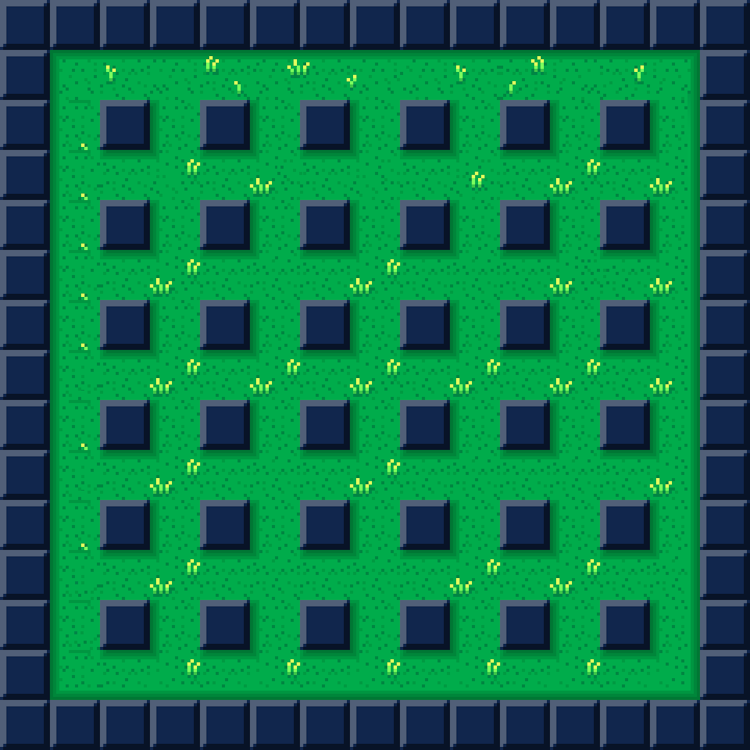
\includegraphics[scale=0.7]{assets/menues/background.png}
    \caption{Ambiente del juego.}
    \label{fig:ambiente del juego}
\end{figure}

\end{frame}
%--------------

\section{Juego Inicialmente}
\begin{frame}
\frametitle{Juego Inicialmente}
\begin{figure}[H]
	\centering
	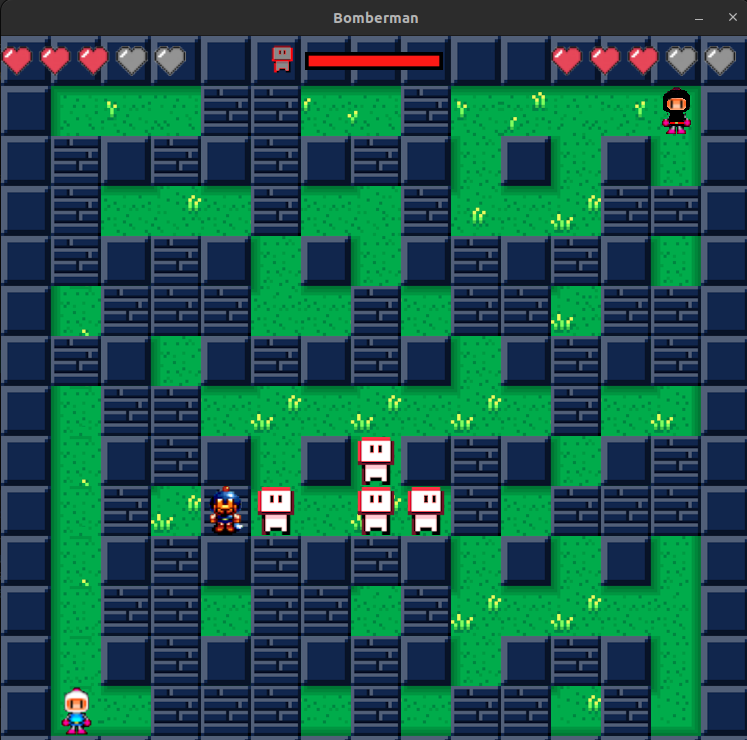
\includegraphics[scale=0.25]{assets/juegoinicia.png}
    \caption{Juego inicialmente.}
    \label{fig:juego inicialmente}
\end{figure}
\end{frame}

%----------------------------------------------------------------------------------------
\begin{frame}
\Huge{\centerline{Fin de presentación}}
\end{frame}

\end{document}
